
We now present \emph{symbolic pairwise lockset analysis}, a novel method for data race analysis in device drivers.  In \S\ref{sec:symbolicpairwise} we describe how the approach works in a semi-formal manner, with respect to a simple concurrent programming model.  In \S\ref{sec:implementation} we explain how we have implemented symbolic pairwise lockset analysis in a practical tool, \whoop, that can be applied directly to driver source code.
%
Our experimental evaluation (\S\ref{evaluation}) demonstrates that the \whoop technique has value as a stand-alone analyzer, and that results from \whoop can be exploited to significantly boost the performance of a more precise symbolic analysis for concurrency, based on context bounding and stratified inlining, offered by the \corral~\cite{lal2012corral} tool; we discuss the latter approach in \S\ref{corral}.

\subsection{Symbolic Pairwise Lockset Analysis}
\label{sec:symbolicpairwise}

Our approach considers, for a given driver, every pair of entry points that can potentially execute concurrently.  For each such pair, we use symbolic verification to check whether it is possible for the pair to race on a shared memory location. We soundly model the effects of additional entry points by treating the driver shared state abstractly: when an entry point reads from the shared state, a nondeterministic value is returned.  Restricting to pairs of entry points, rather than analyzing all entry points simultaneously, exploits the fact that data races occur between pairs of threads and allows our analysis to scale to large drivers.  The trade-off is that a quadratic number of entry point pairs must be checked.  In \S\ref{sec:implementation} we discuss optimizations based on device driver domain knowledge to reduce the number of pairs to some extent.

Symbolic verification of a pair of entry points works by (i) instrumenting each entry point with additional state to record locksets, and (ii) attempting to verify a sequential program that executes the instrumented entry points in sequence and then asserts, for each shared location, that the locksets for each entry point with respect to this location have a non-empty intersection.  Verification of the resulting sequential program can be undertaken using any sound method; in practice we employ the Boogie verification engine~\cite{barnett2006boogie}, which requires procedure specifications and loop invariants to be generated, after which verification conditions~\cite{barnett2005weakest} (VCs) are generated and discharged to an automated theorem prover.

We now detail the approach in a semi-formal manner, in the context of a simple concurrent programming model.

\noindent\textbf{Concurrent Programming Model }
%
We consider a concurrent programming model where an unbounded number of threads execute a set of pre-defined \emph{thread templates}.  At any given point of execution a certain number of threads are active, each thread executing a particular template.  In the context of device drivers, a thread template corresponds to a driver entry point, and multiple instances of the same thread template may execute concurrently, just as multiple invocations of a single driver entry point may be concurrent.  Further threads may start executing at any point during execution; in the context of device drivers this corresponds to the OS invoking additional driver entry points.\footnote{We do \emph{not} consider the case where one thread spawns another thread, which does not occur in the context of drivers; rather we aim to capture the scenario where additional threads are launched by the environment.}  For ease of presentation only, our model does not feature aggregate data types, pointers or dynamic memory allocation.  These \emph{are} handled by our implementation, and in \S\ref{sec:implementation} we discuss interesting practical issues arising from the handling of a full-blown language.

A \emph{concurrent program} is described by a finite set of \emph{shared} variables $\sharedvars$, a finite set of mutexes $\mutexes$, and a finite set of \emph{thread templates}.  A thread template $T$ consists of a finite set of procedures $\procedures{T}$ and a finite set of private variables $\variables{T}$.  A designated procedure $\mainforthread{T} \in \procedures{T}$ denotes the starting point for execution of $T$ by a thread.  Each procedure of $\procedures{T}$ is represented by a control flow graph of basic blocks, where each block contains a sequence of statements.  A basic block either has a single successor or a pair of successors.  In the latter case, an \emph{exit condition} over thread-private variables determines the successor to which control should flow on block exit.

The forms of statements are shown in Figure~\ref{fig:statements}, and include designated statements for reading from and writing to shared variables.  In particular, shared variables may not appear in arbitrary expressions.  This restriction simplifies our presentation of lockset instrumentation, below, and a program that does not satisfy this restriction can be trivially pre-processed into one that does via the introduction of additional private temporary variables to record values read from the shared state.  We do not specify the form of expressions, nor the types of variables, assuming a standard set of data types and operations.

\begin{figure}
\footnotesize
\center
\begin{tabular}{lp{5.5cm}}
\textbf{Statement Form} & \textbf{Notes} \\
\toprule

$x = e;$ & private assignment, where $x \in \variables{T}$ and $e$ is an expression over $\variables{T}$ \\
\midrule

$x = f(\overline{e});$ & procedure call, where $x \in \variables{T}$, $\overline{e}$ is a sequence of expressions over $\variables{T}$, $f$ is the name of a procedure in $\procedures{T}$ \\
\midrule

$s = e;$ & shared write, where $s \in \sharedvars$ and $e$ is an expression over $\variables{T}$ \\
\midrule

$x = s;$ & shared read,  where $x \in \variables{T}$ and $s \in \sharedvars$ \\
\midrule

$\mutexlock{m};$   & mutex lock, where $m \in \mutexes$ \\
\midrule

$\mutexunlock{m};$ & mutex unlock, where $m \in \mutexes$\\
\bottomrule
\end{tabular}
\caption{Forms of statements in our simple programming model}
\label{fig:statements}
\end{figure}

\noindent\textbf{Semantics }
%
Let $\ids$ be an infinite set from which dynamic thread ids will be drawn.  The state of a running concurrent program consists of: a valuation of the shared variables $\sharedvars$; a mapping that associates each mutex in $\mutexes$ with an id from $\ids$, recording which thread currently holds the mutex, or with a special value $\bot \notin \ids$ to indicate that the mutex is not held by any thread; and a list of \emph{threads}.  Each thread consists of an id, drawn from $\ids$, a thread template $T$ an index indicating the next statement of $T$ to be executed by the thread, and a valuation of the thread private variables, $\variables{T}$.  If multiple threads are instances of the same template $T$, then each thread carries a \emph{separate} valuation of the private variables for this template.

At the start of execution the valuation of shared variables is arbitrary, no mutexes are held (i.e.\ each mutex maps to $\bot$), and the list of threads is empty.
%
At any point of execution, a new thread may be added to the list of threads.  This involves selecting a thread template $T$ and an id $i \in \ids$ that has not been previously used during program execution, setting the point of execution for the new thread to be the first statement of $\mainforthread{T}$, and choosing an arbitrary valuation for the private variables $\variables{T}$.
%
We consider a standard interleaving model of concurrency: at any execution point, a thread may execute its current statement, unless that statement has the form $\mutexlock{m}$ and mutex $m$ is already held by some thread.  Executing a statement causes the state of the thread, and the shared state, to be updated in a standard manner.  For example, if a thread following template $T$ executes $s = e$, where $s \in \sharedvars$ and $e$ is an expression over $\variables{T}$, the shared variable valuation is updated so that $s$ has the value determined by evaluating $e$ in the context of the thread's private variable valuation.  Because our interest is in data race analysis for race-free programming, we are not concerned with relaxed memory behavior: race-free programs exhibit only sequentially consistent behaviors.

A thread terminates if it reaches the end of $\mainforthread{T}$; in this case the thread is removed from the list of threads.  Because we are interested in the analysis of device drivers, which are \emph{reactive} concurrent programs, we do not consider the notion of global program termination.

\noindent\textbf{Lockset Instrumentation }
%
For templates $T$ and $U$ (including the possibility that $T$ and $U$ are equal) we want to check whether it is possible for a thread executing $T$ to race with a thread executing $U$, in the presence of arbitrarily many further concurrently executing threads.
%
To this end, we first \emph{instrument} a template $T$ for lockset analysis (see \S\ref{bg:lockset}).  Given an arbitrary symbol $i$, we define the instrumentation of $T$ with respect to $i$, denoted $\instrument{T}{i}$.  There are two aspects to this instrumentation phase: \emph{renaming} and \emph{lockset instrumentation}.

Renaming is straightforward: all occurrences of each private variable $x \in \variables{T}$ used in $T$ are replaced with a renamed variable $\instrument{x}{i}$ in $\instrument{T}{i}$, and every procedure $f \in \procedures{T}$ is renamed (both at its declaration site and at all call sites) to $\instrument{f}{i}$ in $\instrument{T}{i}$.  The purpose of renaming is to ensure that when we analyze a pair of templates, $T$ and $U$, both templates execute distinct procedures and operate on distinct private data.  This is vital in the case where $T$ and $U$ are the same.

\begin{figure}
\footnotesize
\center
\begin{tabular}{ll}
\textbf{Original Statement} & \textbf{Instrumented Statement} \\
\toprule

$s = e;$ & $\hasbeenwritten{i} = \hasbeenwritten{i} \cup \{ s \};$ \\
         & $\lockset{s}{i} = \lockset{s}{i} \cap \currentlockset{i};$ \\
\midrule
         
$x = s;$ & $\hasbeenread{i} = \hasbeenread{i} \cup \{ s \};$ \\
         & $\lockset{s}{i} = \lockset{s}{i} \cap \currentlockset{i};$ \\
         & $\havoc{\instrument{x}{i}};$ \\
\midrule
         
$\mutexlock{m};$   & $\currentlockset{i} = \currentlockset{i} \cup \{ m \};$ \\
\midrule

$\mutexunlock{m};$ & $\currentlockset{i} = \currentlockset{i} \setminus \{ m \};$ \\
\bottomrule
\end{tabular}
\caption{Instrumenting statements for lockset analysis}
\label{fig:instrumentation}
\end{figure}

Lockset instrumentation introduces: sets $\hasbeenread{i} \subseteq \powerset{\sharedvars}$ and $\hasbeenwritten{i} \subseteq \powerset{\sharedvars}$ to track the shared variables that have been read from and written to, respectively, by the thread executing $T$; a current lockset $\currentlockset{i} \subseteq \powerset{\mutexes}$ to record the mutexes currently held by the thread; and, for each shared variable $s \in \sharedvars$, a lockset $\lockset{s}{i}$ to record the mutexes that are consistently held when the thread accesses $s$.
%
The statements of each procedure in $\instrument{T}{i}$ that access shared variables and mutexes are instrumented to manipulate these sets, as shown in Figure~\ref{fig:instrumentation}.  For a shared variable assignment $s = e$, we record in $\hasbeenwritten{i}$ that $s$ has been written to, and update $\lockset{s}{i}$ to eliminate any mutexes that are not currently held (those mutexes that are not in $\currentlockset{i}$).  A shared variable read $x = s$ is instrumented analogously, with an additional $\havockeyword$ command which we discuss below.  Instrumentation of mutex manipulation commands, $\mutexlock{m}$ and $\mutexunlock{m}$, involves updating $\currentlockset{i}$ to add and remove mutex $m$, respectively.

\noindent\textbf{Shared State Abstraction }
%
Recall that while our aim is to perform race analysis for pairs of threads, we must be sure to account for possible side-effects due to other threads that are running concurrently.  The instrumentation of Figure~\ref{fig:instrumentation} achieves this via \emph{nondeterminism}: when reading from a shared variable $s$, a nondeterministic value is returned.  This is reflected by the use of a $\havockeyword$ command, which sets its argument to an arbitrary value.  Because all shared state accesses are abstracted in this fashion, it is possible to completely dispense with the shared variables after the lockset instrumentation has been performed.  As a result, when instrumenting a shared variable write, the effect of the write is not explicitly modeled.

\noindent\textbf{Sequentialisation }
%
The pseudocode of Figure~\ref{fig:sequentialization} shows the sequential program that we analyze in order to prove race-freedom for a pair of thread templates $T$ and $U$. Assuming that $T$ and $U$ have been instrumented using distinct symbols $i$ and $j$, yielding $\instrument{T}{i}$ and $\instrument{U}{j}$, the sequential program operates as follows. First, the read, write and current locksets for $\instrument{T}{i}$ and $\instrument{U}{j}$ are initialized to be empty, and for each shared variable $s$, the locksets $\lockset{s}{i}$ and $\lockset{s}{j}$ are initialized to the full set of mutexes, $\mutexes$.  The main procedures of the instrumented thread templates, $\mainforthread{\instrument{T}{i}}$ and $\mainforthread{\instrument{U}{j}}$, are then executed in turn (the order does not matter, due to renaming). Finally, an assertion checks for consistent use of mutexes: if $s$ is written during execution of $\instrument{T}{i}$ and accessed during execution of $\instrument{U}{j}$, or vice-versa, then the locksets $\lockset{s}{i}$ and $\lockset{s}{j}$ must contain at least one common mutex.

\begin{figure}
\footnotesize
\begin{tabular}{l}
$\currentlockset{i} = \emptyset;$ $\hasbeenread{i} = \emptyset;$ $\hasbeenwritten{i} = \emptyset;$ \\
$\currentlockset{j} = \emptyset;$ $\hasbeenread{j} = \emptyset;$ $\hasbeenwritten{j} = \emptyset;$ \\
\texttt{for} $s \in \sharedvars$ \texttt{do} $\lockset{s}{i} = \mutexes;$ $\lockset{s}{j} = \mutexes;$ \medskip
\\

$\mainforthread{\instrument{T}{i}}();$ \\
$\mainforthread{\instrument{U}{j}}();$ \medskip\\

\texttt{assert} $\forall s \in \sharedvars \; .$ \\

$\quad s \in \hasbeenwritten{i} \cap (\hasbeenread{j} \cup \hasbeenwritten{j}) \vee s \in \hasbeenwritten{j} \cap (\hasbeenread{i} \cup \hasbeenwritten{i}) \implies$ \\

$\quad\quad \lockset{s}{i} \cap \lockset{s}{j} \neq \emptyset;$ \\

\end{tabular}
\caption{The sequential program to be analyzed in order to prove race-freedom for a pair of thread templates}
\label{fig:sequentialization}
\end{figure}

\noindent\textbf{Soundness }
%
We sketch an argument that if the program of Figure~\ref{fig:sequentialization} is correct, it is impossible for a thread executing template $T$ to race with a thread executing template $U$, under the assumption that the threads are guaranteed to terminate. Let us assume that the program of Figure~\ref{fig:sequentialization} is correct, and suppose (by way of contradiction) that a thread executing $T$ can in fact race with a thread executing $U$, on some shared variable $s$.  By our hypothesis that the program of Figure~\ref{fig:sequentialization} is correct, and that the threads terminate, the assertion checked at the end of the program guarantees at least one mutex, say $m$, belongs to both $\lockset{s}{i}$ and $\lockset{s}{j}$.  By the definition of a lockset (and according to the manner in which shared accesses are instrumented in Figure~\ref{fig:instrumentation}), this means that $m$ is held during every access to $s$ by both $\instrument{T}{i}$ and $\instrument{U}{j}$. As a result, $m$ must be unlocked and locked between the two accesses, which contradicts that the pair of accesses is racing.

In the presence of non-termination the assertion at the end of Figure~\ref{fig:sequentialization} may not be reached.  The termination analysis problem for device drivers has been widely studied (see e.g.\ ~\cite{cook2006termination}), and in the remainder of the paper we do not consider termination issues, assuming that the drivers we analyze in our experimental evaluation (see \S\ref{evaluation}) are terminating.

\subsection{Implementation in \whoop}
\label{sec:implementation}

The simple concurrent programming model of \S\ref{sec:symbolicpairwise} is deliberately idealistic to make it easy to describe our symbolic verification technique. In practice, Linux drivers are written in C, we do not know up-front which are the entry points for a driver, drivers do not work with a cleanly specified set of named locks, and rather than having a given set of named shared variables, we have arbitrary memory accesses via pointers. We now explain how we have taken the conceptual ideas from \S\ref{sec:symbolicpairwise} and used them to build \whoop\footnote{\url{https://github.com/pdeligia/whoop}}, a practical, fully automatic tool for detecting data races in drivers.

\begin{figure*}
\centering
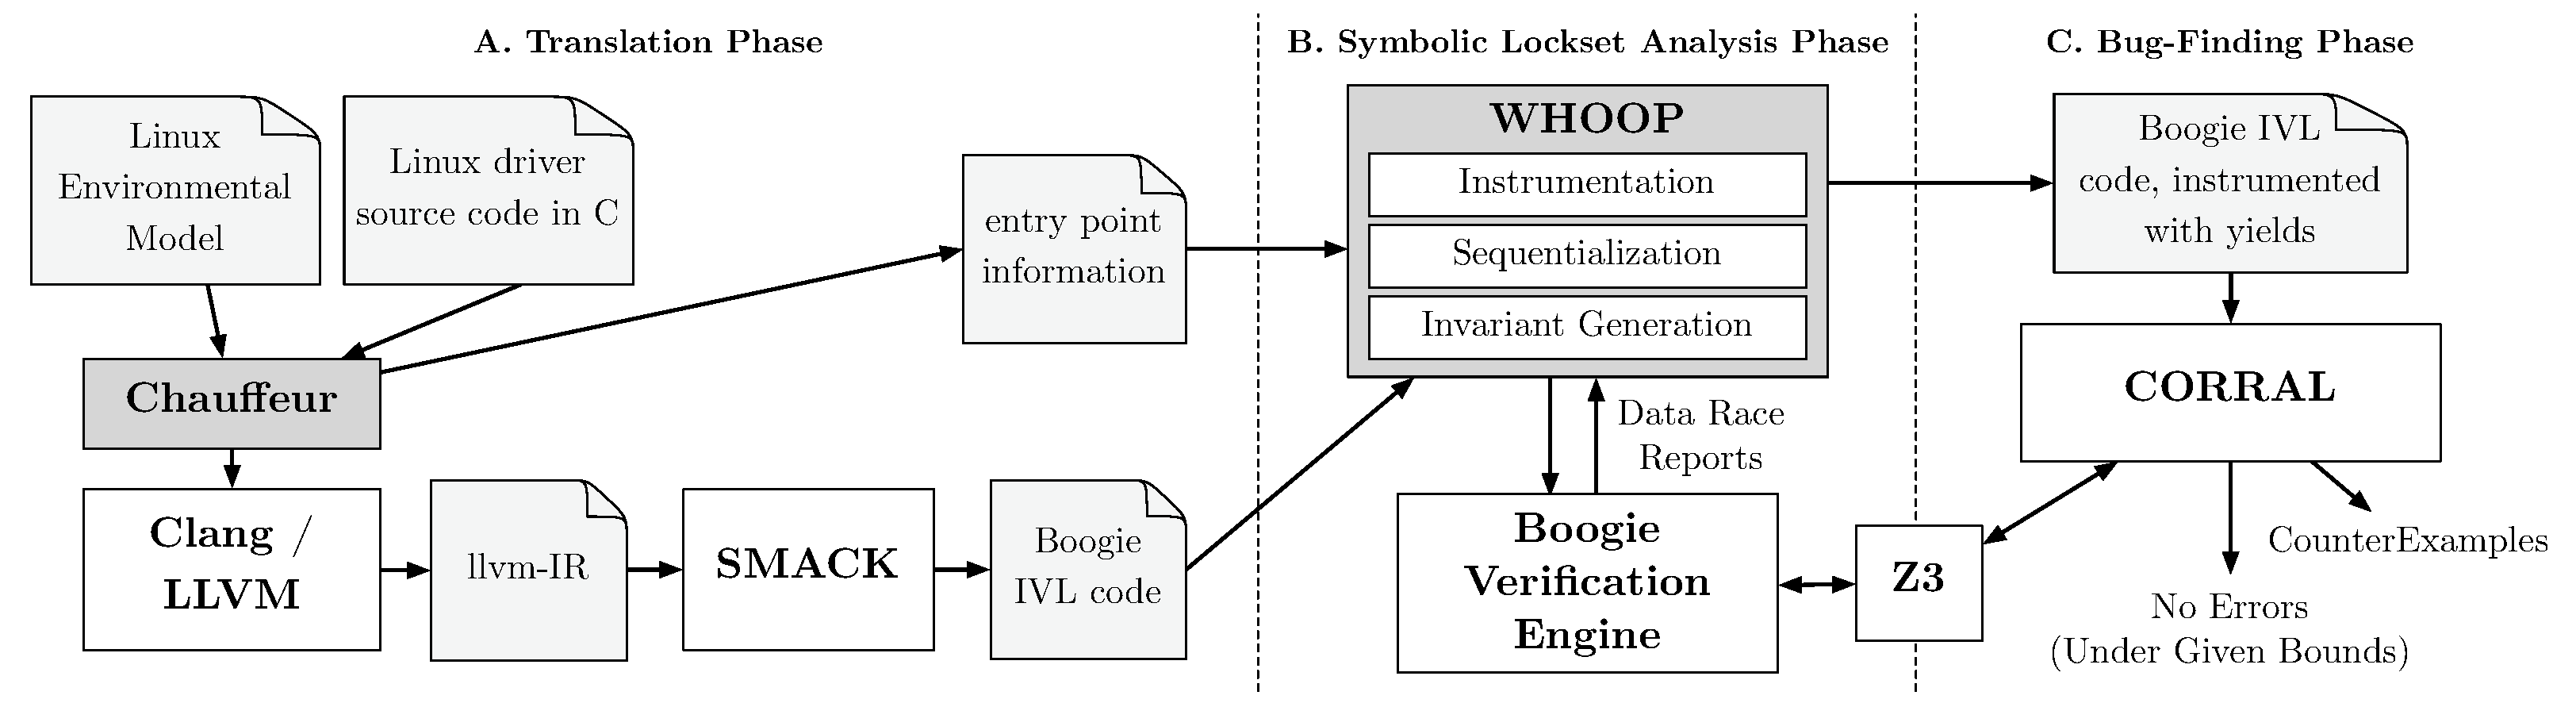
\includegraphics[width=.99\linewidth]{img/whoop.pdf}
\caption{The \whoop architecture, empowered by state-of-the-art compilation (Clang/LLVM and SMACK) and verification (Boogie and \corral) tools}
\label{fig:whoop}
\end{figure*}

\noindent\textbf{Architecture }
%
Figure~\ref{fig:whoop} depicts the \whoop toolchain. Initially, \whoop accepts a Linux driver written in C, together with an environmental model\footnote{This consists of stub header files modeling relevant Linux kernel APIs.} that is required to ``close'' the driver and allow it to be subsequently analyzed for data races. Both the driver and the Linux model are passed to the translation phase of \whoop (see Figure~\ref{fig:whoop} -- A), which uses three LLVM\footnote{\url{http://llvm.org}}-based tools, Chauffeur\footnote{\url{https://github.com/mc-imperial/chauffeur}}, Clang\footnote{\url{http://clang.llvm.org}} and SMACK\footnote{\url{https://github.com/smackers/smack}}~\cite{rakamaric2014smack}, to translate the original driver into an abstract program written in the Boogie intermediate verification language (IVL)~\cite{deline2005boogiepl}, a simple imperative language with well-defined semantics that is used as the input to a number of cutting-edge verifiers (e.g.\ Boogie and \corral).

Next, \whoop instruments and sequentializes the program to perform symbolic pairwise lockset analysis (see Figure~\ref{fig:whoop} -- B and \S\ref{sec:symbolicpairwise}) using the Boogie verification engine. After the verification phase ends, \whoop can exploit any inferred race-freedom guarantees to accelerate precise race-checking with \corral (see Figure~\ref{fig:whoop} -- C and \S\ref{corral}).

We engineered the Chauffeur and \whoop components of our toolchain (denoted with grey boxes in Figure~\ref{fig:whoop}).  For the remaining components, we were able to reuse industrial-strength tools that are robust and battle-proven via their use in many complex software projects.

\noindent\textbf{Extracting Entry Point Information }
%
Chauffeur is a Clang-based frontend that traverses the abstract syntax tree (AST) of the original driver (using a Clang visitor pass) and extracts all entry point identifier names, together with the identifier names of their corresponding kernel API functions. Linux drivers define entry points in a standard way (see Figure~\ref{fig:entrypoints} for an example of how the generic\_nvram driver defines the entry points for the \texttt{file\_operations} API); Chauffeur identifies these definitions in the AST and outputs the relevant information in an XML file, which is subsequently parsed by \whoop and used during the instrumentation.

\begin{figure}[t]
\begin{lstlisting}
const struct file_operations nvram_fops = {
  .llseek = nvram_llseek,
  .read = read_nvram,
  .write = write_nvram,
  .unlocked_ioctl = nvram_unlocked_ioctl,
};
\end{lstlisting}
\caption{Entry points definitions in the generic\_nvram driver}
\label{fig:entrypoints}
\end{figure}

\noindent\textbf{Translation for Verification }
%
Next, the driver is compiled by Clang to LLVM-IR~\cite{lattner2004llvm}, a low-level assembly-like language in single static assignment (SSA) form. Function calls (e.g.\ for locking and unlocking) are preserved in this translation, which is useful for our lockset instrumentation.

SMACK then translates the driver from LLVM-IR to Boogie IVL, which is the input language of \whoop. An important feature of SMACK is that it leverages the pointer-alias analyses of LLVM to efficiently model the heap manipulation operations of C programs in Boogie IVL. This means that \whoop does not need to directly deal with pointers and alias analysis, a hard problem on its own, allowing us to reuse robust existing techniques and focus instead on verification efforts.

To achieve scalability, SMACK uses a \emph{split} memory model that exploits an alias analysis to soundly partition memory locations into non-overlapping equivalence classes that do not alias. This has been shown to lead to more tractable verification compared with a \emph{monolithic} model where the heap is considered to be an array of bytes~\cite{rakamaric2009scalable}. The split memory model is based on \emph{memory regions}, which are maps of integers that model the heap. A benefit of using this model is that distinct memory regions denote disjoint sections of the heap. We leverage this knowledge inside \whoop to guide and optimize our lockset instrumentation and analysis, and to create a fine-grained context-switch instrumentation as discussed in \S\ref{corral}.

\noindent\textbf{Identifying Locks }
%
When the instrumentation phase begins, \whoop performs an inter-procedural static analysis (on the Boogie IVL source code of each entry point) to identify all available locks and rewrite each one (both at declaration and at all access sites) to a unique constant Boogie variable. The reason behind this transformation, is that representing all locks statically, instead of their original SMACK pointer-based representation, helps \whoop perform various internal instrumentation and optimization passes.
%
Currently, \whoop only supports mutexes and spinlocks that are available in the Linux kernel APIs. However, it is relatively easy to enhance our tool with knowledge of other locking primitives. If \whoop cannot infer a lock, e.g. because it was created dynamically or was indexed from an array of locks, it will exit with a warning. The are two reasons behind this: (i) it is arguably hard to detect such locks using static analysis; and (ii) a small, fixed number of locks is advocated by Linux experts as good practice when developing drivers~\cite{corbet2005linux}.

\noindent\textbf{Watchdog Race-Checking Instrumentation }
%
Data race detection is performed by introducing sets containing the locks that are consistently held by each shared variable and sets containing all shared variables that are read and written (see \S\ref{sec:symbolicpairwise} and the instrumentation of Figure~\ref{fig:instrumentation}). These sets can be modeled directly in Boogie as characteristic functions, using maps. However, this requires the use of quantifiers to express properties related to set contents.  For instance, to express that a set $X$ of elements of type $A$ is empty, where $X$ is represented as a map from $A$ to $\mathsf{Bool}$, we would require the quantified expression $\forall a : A : \neg X[a]$.  It is well known that automated theorem proving in the presence of quantified constraints is challenging, and that theorem provers such as Z3~\cite{de2008z3} are often much more effective when quantifiers are avoided.  

To avoid quantifiers and the associated theorem proving burden, we use instead a \emph{watchdog race-checking instrumentation}, adapted from~\cite{bardsley2014engineering}.  Suppose we are analyzing entry points $T$ and $U$, and that after translation into Boogie these entry points share a common memory region, $\mathit{MR}$.  When analyzing $T$ and $U$ for races, we introduce an unconstrained symbolic constant $\mathit{watched}_{\mathit{MR}}$, representing some unspecified index into $\mathit{MR}$; we call this the \emph{watched offset} for $\mathit{MR}$.  We then attempt to prove that it is impossible for $T$ and $U$ to race on $\mathit{MR}$ at index $\mathit{watched}_{\mathit{MR}}$.  If we can succeed in proving this, we know that $T$ and $U$ must be race-free for the \emph{whole} of $\mathit{MR}$, since the watched offset was arbitrary.  This technique of choosing an arbitrary index to analyze for each map manipulated by an entry point pair can be seen as a form of quantifier elimination: rather than asking the underlying theorem prover to reason for all indices of $\mathit{MR}$, in a quantified manner, we eliminate the quantifier in our encoding, and instead ask the theorem prover to reason about a single, but arbitrary, index of $\mathit{MR}$.

\noindent\textbf{Generating Loop and Procedure Summaries }
%
Early in the development of \whoop, we experimented with analyzing recursion-free drivers using full inlining.  We found that this did not scale to large drivers: when we tried to apply \whoop to the r8169 ethernet driver (see \S\ref{evaluation}), we quickly exhausted the memory limits of our experimental platform as the driver exhibited recursion, which cannot be fully inlined.

To make our analysis scalable without sacrificing precision, and to cater for recursion, we use the Houdini~\cite{flanagan2001houdini} invariant inference algorithm to automatically compute summaries (pre- and post-conditions and loop invariants) from a pool of \emph{candidate} invariants.  Given a pool of candidates, Houdini repeatedly attempts to verify each procedure with respect to its current candidate summary.  If verification fails due to an incorrect candidate, this candidate is discarded.  The process repeats until a fixpoint is reached, whereby the largest conjunction of the candidate invariants that can be proven to hold remains.  The remaining candidates, which are indeed invariants, can then be assumed during further analysis of the program.

Houdini does not generate the initial pool of candidates: \whoop generates them using a set of heuristics, and passes them to Houdini as a starting point.  The idea is to automatically generate likely program invariants based on syntactic patterns extracted from an inter-procedural pass over the code for an entry point.  We give two examples; for clarity we use notation from the simple shared variable concurrent programming model of \S\ref{sec:symbolicpairwise}.  If we observe syntactically that procedure $f$ of entry point $T$ may write to, but does not read from, shared variable $s$, then when instrumenting $T$ with symbol $i$, we guess $s \in \hasbeenwritten{i}$ and $s \notin\hasbeenread{i}$ as postconditions for $\instrument{f}{i}$.  These guesses may be incorrect, for instance if the potential write to $s$ turns out to be in dead code, or if a read from $s$ has already been issued on entry to $\instrument{f}{i}$.  Similarly, if syntactic analysis indicates that $f$ may unlock mutex $m$, we guess $m \notin \currentlockset{i}$ as a postcondition for $\instrument{f}{i}$; this guess may be wrong, e.g.\ if the unlock operation is not reachable or if a subsequent lock operation acquires the mutex again.  We stress that guessing incorrect candidate invariants does not compromise the soundness of verification: \whoop is free to speculatively generate candidates that are later deemed to be incorrect, and thus discarded, by Houdini.  The balance we try to strike is to have \whoop generate sufficient candidates to enable precise lockset analysis, without generating so many candidates that the speed of the Houdini algorithm is prohibitively slow.

In practice, the candidates are generated at the Boogie IVL level, with respect to SMACK-generated memory regions and referencing the auxiliary variables introduced by our watchdog race-checking instrumentation.

\noindent\textbf{Verification and Error Reporting }
%
For each pair of entry points, the instrumented sequential program, equipped with procedure and loop summaries, is sent to the Boogie verification engine. Boogie generates a VC, for each procedure in the program, and discharges it to the Z3~\cite{de2008z3} theorem prover.  In particular, the verification for the root-level procedure, encoding the sequential program sketched in Figure~\ref{fig:sequentialization}, encodes the race-freedom check for the entry point pair. Successful verification implies that the entry point pair is free of data races, while an error (i.e.\ counterexample) denotes a \emph{potential} data race and is reported to the user. To improve usability, \whoop has a built-in error reporter that matches counterexamples to source code. The following is a race that \whoop found and reported for the example of Figure~\ref{fig:data_race_example}: 

\begin{lstlisting}[keywordstyle=\ttfamily]
generic_nvram.c: error: potential read-write race:
  read by entry point nvram_llseek, generic_nvram.c:54:2
    return file->f_pos;
  write by entry point nvram_llseek, generic_nvram.c:53:2
    file->f_pos = offset;
\end{lstlisting}

Because a driver is processed by Clang and SMACK during the translation from C to Boogie IVL, significant engineering effort was required to map Boogie-level errors back to original source code locations.

\noindent\textbf{Optimizations }
%
We have implemented various optimizations to increase the precision and performance of \whoop.  We comment on the two most effective optimizations.

First, we enriched \whoop with information regarding \emph{kernel-imposed serialization}, to increase precision. The Linux kernel can serialize calls to entry points, thus forcing them to run sequentially with each other. As an example, a large number of networking entry points are mutually serialized with RTNL, a network-specific kernel lock. We discovered this when we first analyzed the r8169 driver (see \S\ref{evaluation}) and \whoop reported many races between a number of networking entry points; when we investigated the source of these races, we found out that these entry points could not race in reality because of RTNL. \whoop exploits this knowledge and does not create pairs for entry points that are serialized by the kernel. This is an ongoing manual effort: the more drivers we study, the more such properties we discover, which we can then exploit to make \whoop more precise. Currently, this information is hard-coded inside \whoop. In the future, we plan to provide a configuration file where the user can denote such kernel specific information.

Second, we soundly reduce the number of memory regions that are analyzed for races.  If memory region $\mathit{MR}$ is accessed by only one entry point in a pair then, trivially, the pair cannot race on $\mathit{MR}$.  We thus disable lockset analysis for $\mathit{MR}$.  This can reduce the complexity of VCs that need to be solved by the theorem prover, speeding up the verification process.

\noindent\textbf{Practical Assumptions Related to Soundness}
%
\whoop is ``soundy''\footnote{\url{http://soundiness.org/}}~\cite{soundiness}: it aims in principle to perform a sound analysis that can prove absence of races, but suffers from some known sources of unsoundness, which we now comment on.

We assume that the formal parameters of an entry point do not alias, and thus cannot race. This is a potentially unsound feature that can be turned off using a command line option, but without this assumption the false alarm rate of \whoop is very high. In our experience so far, we have not missed any races by assuming non-overlapping parameters.  We also rely on the soundness of our best-effort environmental model, and on exploiting domain-specific knowledge related to entry point serialization by the Linux kernel.

As well as inheriting soundness issues arising from currently unknown bugs in \whoop and in the external tools that \whoop relies on, we acknowledge that: (i) SMACK is subject to sources of unsoundness, e.g.\ it models integers as an infinite set (rather than as a finite set of bit-vectors), and its memory model can potentially be unsound in (typically rare) situations where programs use unaligned byte-level memory accesses; and (ii) that the combination of Clang and SMACK commits our approach to specific choices related to undefined and implementation-defined aspects of the C language when translating to Boogie.  However, \whoop makes no fundamental assumptions related to these translation decisions, meaning that a more accurate C-to-Boogie translation would automatically lead to a more accurate analysis with \whoop.

\noindent\textbf{Limitations }
%
As a lockset analyzer, \whoop can be imprecise because a violation of the locking discipline does not always correspond to a real race (e.g.\ when lockfree synchronization is used). \whoop also over-approximates drivers, which can be another source of imprecision. Furthermore, the tool does not check for dynamically created locks or for locks provided by external libraries, although the later could be addressed by providing a mechanism for users to declare custom locks. We also do not currently treat interrupt handlers in a special way; we just assume that they can execute concurrently with any entry point. One way to address this is to model interrupt-specific kernel functions (e.g. for enabling/disabling interrupts).

Another limitation of \whoop is that it is unable to verify drivers designed to be accessed by only a single process at a time. This \emph{single-open device}~\cite{corbet2005linux} mode can be enforced by atomically testing (at the beginning of an entry point) a flag that indicates device availability: if the flag is set to true, then the checking entry point executes, else it blocks. Because \whoop performs pair-wise analysis, it over-approximates this flag, and thus can falsely report a pair as racy. However,~\cite{corbet2005linux} advises against serializing drivers in this way, as it hinders user ingenuity (e.g.\ a user might expect that a device can be accessed concurrently for performance). Because this serialization is considered bad practice, we burden the developer with disregarding any related false bug reports.

Statically analyzing drivers requires to ``close'' the environment by abstracting away the low-level implementation details. To this end, we developed a simple model for the Linux kernel that consists of (nondeterministic) stub functions. A limitation of our model is that it can, and will, ultimately result in false positives. However, we currently only focus on finding data races, and thus can get away with over-approximating a lot of the underlying kernel functionality, without losing too much precision. Making our model more precise is an ongoing manual effort, but requires Linux expertise. We argue that further work on the model is orthogonal to the contributions of this paper. Also, even if our symbolic analysis results in false positives, \whoop can still use the results to significantly speedup a more precise bug-finder, as seen in \S\ref{corral} and \S\ref{evaluation}.
